\begin{frame}{Beacon Usecases}
    % \tikzstyle{decision} = [diamond, draw, fill=blue!20,
    % text width=5em, text badly centered, inner sep=0pt]
% \tikzstyle{block} = [rectangle, draw, fill=blue!20,
    % text width=5em, text centered, rounded corners, minimum height=4em]
% \begin{tikzpicture}[auto]
    % \scriptsize
    % % Place nodes
    % \node [block] (init)                            { start};
    % \node [decision, right of=init] (crypto)        { Is it for cryptography?};
    % \node [decision, right of=crypto] (trust)       { Do you need users to trust the randomness?};
    % \node [decision, right of=trust] (third)        { Do you blindly trust a 3rd party?};
    % \node [decision, below of=third] (available)    { Are you operating in a public setting?};
    % \node [block, below of=trust] (dont)            { Don't use a beacon};
    % \node [block, right of=third] (autocratic)      { Use an \emph                                 { Autocratic Collector}};
    % \node [block, right of=available] (transparent) { Use a \emph                                  { Transparent Authority}};
    % \node [block, below of=transparent] (mpc)       { Use a \emph                                  { Specialized MPC}};
    % % Draw edges
    % \path [arrow] (init) -- (crypto);
    % \path [arrow] (crypto) |- node {Yes} (dont);
    % \path [arrow] (crypto) -- node {No} (trust);
    % \path [arrow] (trust) -- node {No} (dont);
    % \path [arrow] (trust) -- node {Yes} (third);
    % \path [arrow] (third) -- node {Yes} (autocratic);
    % \path [arrow] (third) -- node {No} (available);
    % \path [arrow] (available) |- node {No} (mpc);
    % \path [arrow] (available) -- node {Yes} (transparent);
% \end{tikzpicture}
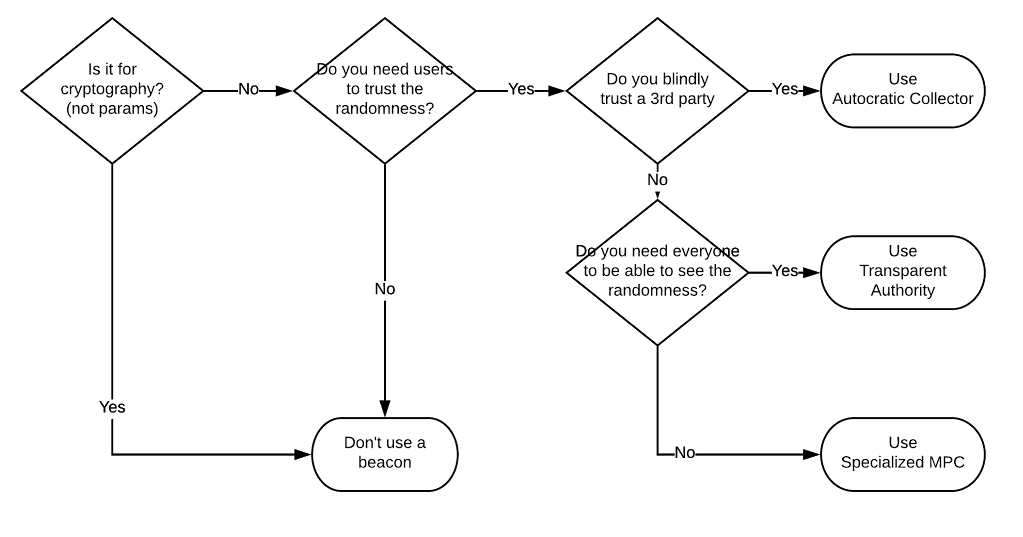
\includegraphics[width=\textwidth]{figures/beaconflow.png}
\end{frame}
    \note{
        \begin{itemize}
            \item Figure to explain proper beacon usecases
            \item Permissioned usecase - smaller community, businesses for randomness or even fair contract signing.
        \end{itemize}}
